\section{Data}

\subsection{The Market and Demand}

The middle European electricity market cannot be restricted to one country only. However, we focus on Germany as the four biggest Players (EoN, RWE, Vattenfal and EnBW) and the most important electricity exchange in the Region, the EEX are situated there. There are, however, significant import capacities from the neighboring countries (see \cite{Ellersdorfer2005} p. 30). Other electricity Exchanges are the EXAA in Austria, the APX in The Netherlands and the Powernext in France. Apart from energy exchanges, there are OTC Markets as well for which data are hard to get. However, prices at the electricity exchanges are generally regarded as a reliable price signal for the OTC Market. \cite{Holler2006} compare OTC prices and prices from the exchanges (EEX and EXAA) in Austria and Germany and conclude that both prices seem to reflect one market in the respective countries. Furthermore, they look at correlations between market prices at the different exchanges and come to the conclusion, that prices at the EEX, EXAA and Powernext are highly correlated. However, only about four percent of the French electricity consumption is traded at the spot market and the whole French industry is heavily dominated by EDF which casts some doubt on whether there is a working electricity market in France. This is why we do not model France as a strategic part of the market which does not mean that research on that topic would not be interesting. Furthermore, the only countries where transmission lines are not congested at the moment, are Germany and Austria\footnote{For an overview of current cross-boarder congestion management methods in europe, see www.etso-net.org.} which is why we restrict our analysis to the two latter countries.
\begin{figure}[h]
\centering
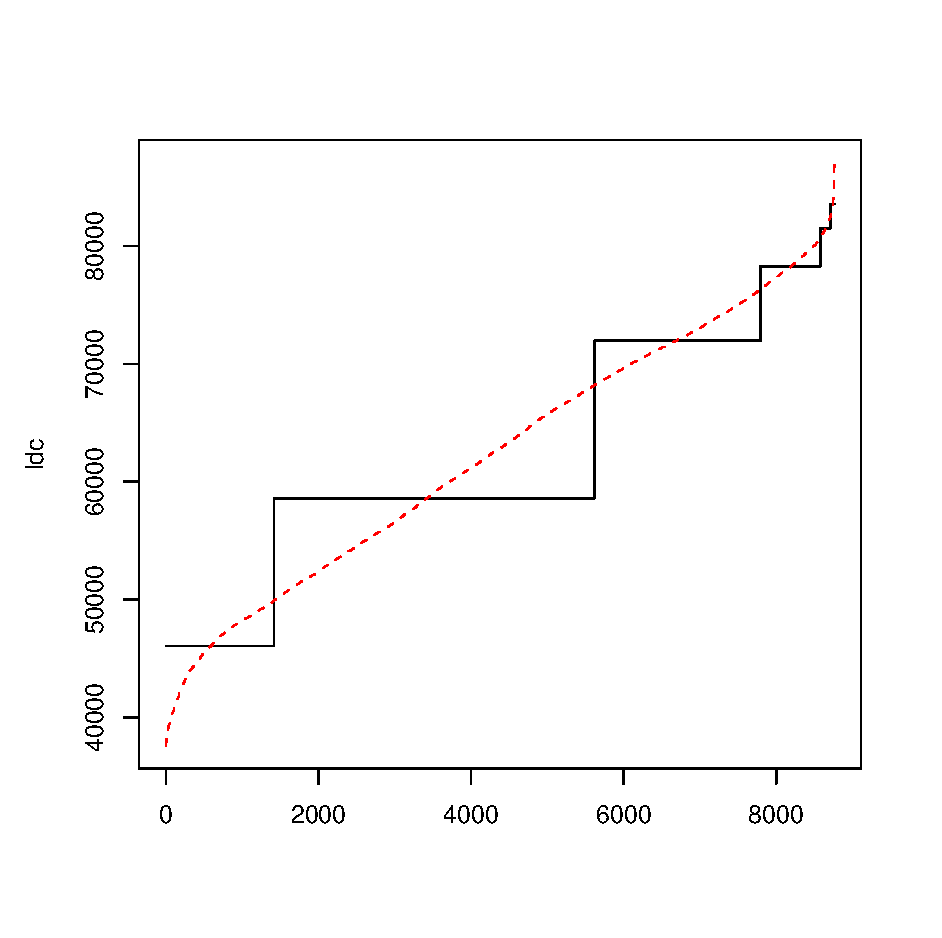
\includegraphics[width=.5\textwidth]{data/ldc}
      \label{fig:ldc}
      \caption{Load Duration Curve in MW for Austria and Germany}
      source: UCTE\footnote{http://www.ucte.org/}
\end{figure}
Figure \ref{fig:ldc} shows the load duration curve for Germany and Austria. It can be seen that there are a few extreme demand spikes and normal values between roughly 80.000 and 40.000 MWh.. To get a better picture of the market, in Figure \ref{fig:korrelation}, hourly Prices from the EEX were plotted against total hourly electricity load in the economy. The correlation is evident. Furthermore, there seems to be an upper bound to capacity which leads prices to explode if that bound is approached. Of course, quantity is not the only factor to explain prices and so there is uncertainty associated with our model. It could well be that demand in the neighboring countries is lower than expected during a high demand period in Germany and so this free capacities dampen the price spike at the EEX. All these uncertain other developments shall be accounted for by our approximated load duration curve which tells us how often the market is in which state during a year. An interesting thing to note is that if we plot prices and quantities at the EEX there seems to be no correlation at all. This is another sign that the exchange just does not cover the whole market and that there is a closely related OTC market which, together with the exchange forms the actual market for electricity.

\begin{figure}[h]
\centering
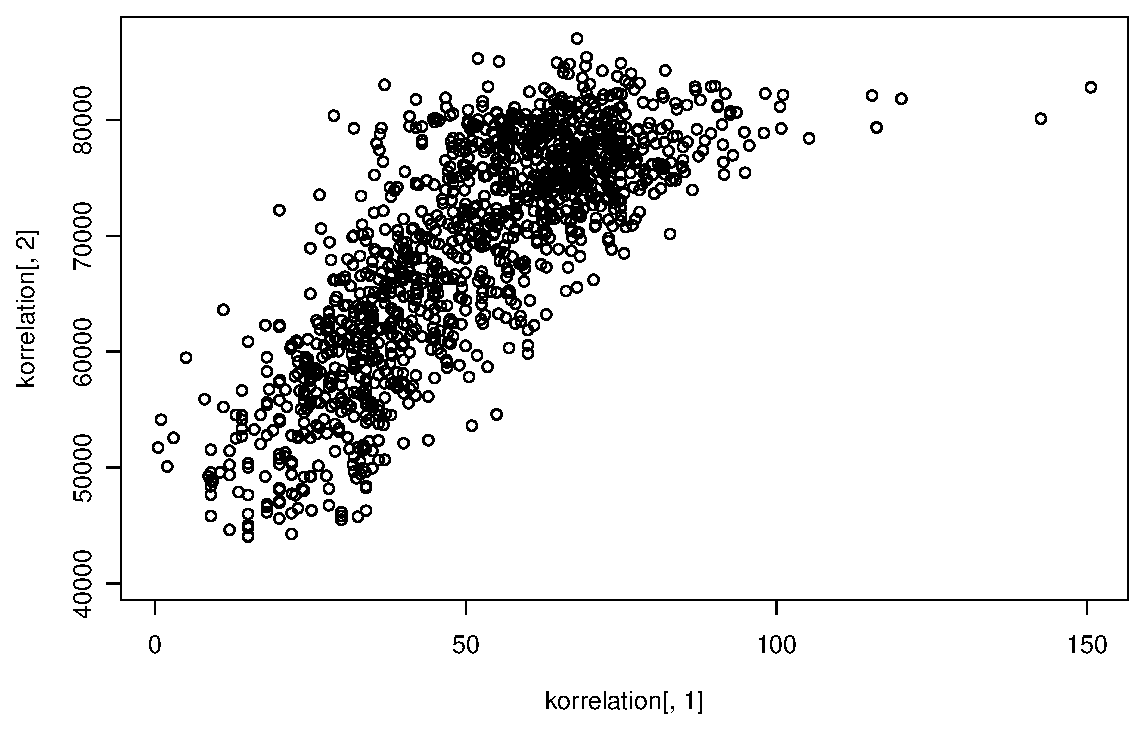
\includegraphics[width=.5\textwidth]{data/korrelation}
      \label{fig:korrelation}
      \caption{Load Duration Curve and our approximation for Austria and Germany}
      source: UCTE and EEX \footnote{http://www.ucte.org/; http://www.eex.com/}
\end{figure}

To account for different states of the market we separated the price-quantity combinaitons which occurred within a year by prices. As can be seen in Table \ref{tab:demand}, markets with extremely high prices occur only seldomly and prices between 20 and 40 are most common. For each of the six states in which the market might be we created linear demand functions based on average prices and quantities in theese states. Average quantities can also be seen in figure \ref{fig:ldc} where the real load duration curve is compared with our approximation. Note that in order to account for price spikes we model the high-price end of the market quite accurately. To construct demand curves, \cite{Neuhoff2005} use a demand elasticity of 0.1, whereby \cite{Genc2007} argue that 0.2 is more commonly used to simulate the electricity market. As we have a more long run focus we decided to use 0.2 as in the long run, elasticity is higher. It might be argued, that in an electricity market, there is no elasticity anyway as maybe only a very few industrial clients reduce their demand as prices rise. Responding to this, \cite{Bushnell2003} notes that imports and exports provide some elasticity.

\begin{table}
\begin{center}
\begin{tabular}{lllll}
\hline
 & \multicolumn{1}{c}{Occurance} & \multicolumn{1}{c}{average price} & \multicolumn{1}{c}{average quantity} &  \\ 
 & \multicolumn{1}{c}{per year} & \multicolumn{1}{c}{(EUR)} & \multicolumn{1}{c}{(MWh)} &  \\ 
 \hline
$>$ 100 & \multicolumn{1}{c}{46} & \multicolumn{1}{c}{128} & \multicolumn{1}{c}{83558} &  \\ 
between 80 and 100 & \multicolumn{1}{c}{134} & \multicolumn{1}{c}{86} & \multicolumn{1}{c}{81493} &  \\ 
between 60 and 80 & \multicolumn{1}{c}{788} & \multicolumn{1}{c}{68} & \multicolumn{1}{c}{78256} &  \\ 
between 40 and 60 & \multicolumn{1}{c}{2174} & \multicolumn{1}{c}{49} & \multicolumn{1}{c}{71956} &  \\ 
between 20 and 40 & \multicolumn{1}{c}{4201} & \multicolumn{1}{c}{30} & \multicolumn{1}{c}{58578} &  \\ 
below 20 & \multicolumn{1}{c}{1417} & \multicolumn{1}{c}{14} & \multicolumn{1}{c}{42627} &  \\
\hline
 & \multicolumn{1}{c}{8760} &  &  &  \\ 
 \hline
\end{tabular}
\end{center}
\label{tab:demand}
\caption{market segments}
\begin{center}
source: UCTE and EEX \footnote{http://www.ucte.org/; http://www.eex.com/}
\end{center}    
\end{table}

\subsection{Supply}

Data concerning the short run marginal costs and investment costs per MWh were obtained from \cite[p.46]{Auer2006} and are shown in table \ref{tab:costs}. For pump storage plants we used the real option value of peak load electricity which we approximated by the average option price for peak load electricity at the EEX in the year 2006. We do not provide fixed costs for pump hydropower and oil plants. In the case of hydropower plants construction costs depend heavily on the respective sites and so such costs are hard to estimate. Furthermore, all available sites for significant hydropower capacities in central europe seem to be occupied already. Oil fired plants are not considered a relevent investment option because oil prices are just too high. The fixed investment costs we use could also be interpreted as a discounted present value of future yearly costs of capital so our analysis is general concerning this point.

Apart from the dominant players, there is a competitive fringe as well which is a price taker as he cannot influence market prices due to it�s small size. \cite{Neuhoff2005} notes that fringe players could also be modeled to respond to output choices of the strategic players, however we do not account for that.

\begin{table}
\begin{center}

\begin{tabular}{rrr}
\hline
           & Variable Costs & Investment Costs \\

           & (EURO/MWh) & EURO je MWh \\
\hline
     Hydro &        7.6 &    3500000 \\

   Nuclear &        9.5 &    1841000 \\

   Lignite &       10.6 &    1074000 \\

 Hard Coal &       16.1 &     971000 \\

CCGT &       33.5 &     460000 \\

Oil & 44            &   n.a \\
%Gas Turbines &       53.8 &     332000 \\

Pump Hydro &         80 &       n.a. \\
\hline
\end{tabular}  

\end{center}
\label{tab:costs}
\caption{variable and fixed costs}
\begin{center}
source: \cite{Auer2006}
\end{center}
\end{table}

%For cost data see also \cite{Kuester2007}.

Installed Capacities of all dominant players and the competitive fringe were taken from \cite{Ellersdorfer2005} and are given in table \ref{tab:capacities}. Please note that the capacities of the Austrian players are considered to be non-strategic as well.t

%It is striking, that most of the renewable capacities are controlled by fringe players. We constructed a supply curve for the competitive fringe by using the following fourth order polynomial approximation (\ref{eq:19}) of the step wise marginal cost function. The approximation, which weights were obtainded by an OLS Method is illustrated in figure \ref{fig:fringe}.

%\begin{equation}
%  \label{eq:19}
%  C^t_{i} = c_1 + c_2 (\sum_{k=1}^m q^{t,s}_{i,m}) + c_3(\sum_{k=1}^m q^{t,s}_{i,m})^2 + c_4(\sum_{k=1}^m q^{t,s}_{i,m})^3 + (\sum_{k=1}^m q^{t,s}_{i,m})^4
% \end{equation}
 
%\begin{figure}[h]
%\centering
%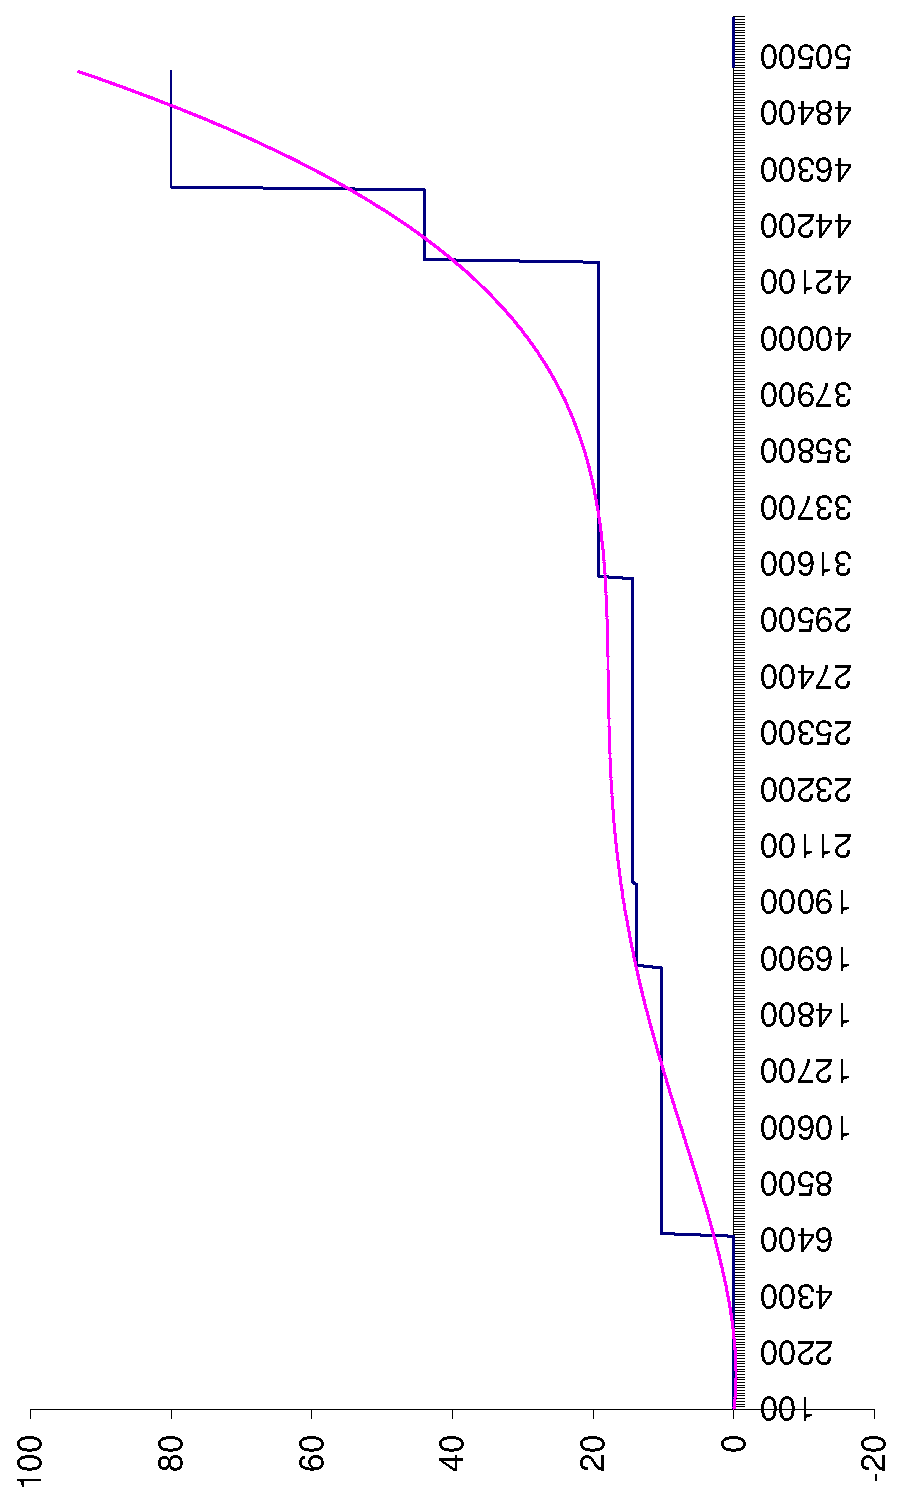
\includegraphics[width=.3\textwidth, angle=-90 ]{data/fringe_costs}
%      \label{fig:fringe}
%      \caption{polynomial approximation of fringe marginal costs (in EUR and MW)}
%      source: own calculations
%\end{figure}

%For the strategic players however, we cannot use such a simple method because we want to account for the effect of investments in different technologies. The following formulations provide cost functions which are continuous, differentiable and provide a reasonable approximation of step wise cost functions.

%\begin{equation}
%  \label{eq:20}
%		C^{}_{h,k} =  c_k * q_{k,h} + b (\frac{K_k}{(\phi+1)}\frac{q_{k,h}}{K_k})^\phi
% \end{equation}

%\begin{equation}
%  \label{eq:20}
%		MC^{t}_{i} =  c_m + b \frac{q^{t,s}_{i,m}}{K^{t,s}_{i,m}}^\phi
% \end{equation}

%\begin{equation}
%  \label{eq:20}
%		C^{t}_{i} = \sum_{k=1}^{m} q^{t,s}_{i,m} c_m + \frac{1}{(K^{t,s}_{i,m}-q^{t,s}_{i,m})}
% \end{equation}

%With marginal costs

%\begin{equation}
%  \label{eq:20}
%		C^{t}_{i} = \sum_{k=1}^{m} c_m + \frac{1}{(K^{t,s}_{i,m}-q^{t,s}_{i,m})^2}
% \end{equation}





Show that Austrian players are fringe? 

Long term structure of plant parks.

How does the resulting plant park structure look like, if firms actually play two-stage open or closed-looped games and other possible market structures (perfect competition, Betrand). 

How could the current market structures look like one long term step ahead (in ten years from now, one investment cycle).

Welfare implications from different market structures.

Implications of capacity markets.

